\documentclass{beamer}
\usepackage[utf8]{inputenc}
\usepackage[T1]{fontenc}
\usepackage{lmodern}
\usepackage{tikz}
\usetikzlibrary{snakes}
\usetikzlibrary{decorations.pathreplacing}
\usepackage[absolute,overlay]{textpos}
\usepackage{booktabs}
\usepackage{ulem}
\usepackage{array}

\title{Meilenstein 3}
\author{Projektgruppe FastSense}
\date{25. Januar 2021}

\usecolortheme{seahorse}
\definecolor{dark}{rgb}{0, 0.1, 0.3}
\definecolor{light}{rgb}{0.9, 0.933, 1}
\definecolor{hw}{rgb}{0.8, 1, 0.9}
\definecolor{red}{rgb}{1, 0, 0}
\definecolor{yellow}{rgb}{1, 1, 0}
\definecolor{green}{rgb}{0, 1, 0}
\definecolor{cyan}{rgb}{0, 1, 1}
\definecolor{blue}{rgb}{0, 0, 1}
\definecolor{magenta}{rgb}{1, 0, 1}
\definecolor{grey}{rgb}{0.8, 0.8, 0.8}
\setbeamercolor{normal text}{fg=black}
\setbeamercolor{structure}{fg=dark}
\setbeamercolor{footline}{fg=black}
\setbeamercolor{frametitle}{fg=light,bg=dark}
\setbeamertemplate{itemize items}[circle]
\beamertemplatenavigationsymbolsempty
\addtobeamertemplate{navigation symbols}{}{
    \usebeamerfont{footline}
    \usebeamercolor[fg]{footline}
    {\footnotesize \insertframenumber\\\vspace{0.15cm}}
}
\setbeamertemplate{title page}{
\insertauthor\\\vspace{0.5cm}
\begin{LARGE}\textbf{\inserttitle}\end{LARGE}\\\vspace{0.5cm}
\insertdate
}

\begin{document}

{\setbeamertemplate{navigation symbols}{}
\begin{frame}
\titlepage
\end{frame}}

\begin{frame}{Inhalt}
\tableofcontents
\begin{textblock*}{1cm}(0cm,3.2cm)
\begin{tikzpicture}
\draw [white] (0, 2.35) rectangle +(1, 1); % Hier den y-Wert anpassen, falls sich das Inhaltsverzeichnis noch ändert
\draw [light, ultra thick] (1, 0) -- (7, 0);
\node [right, dark] at (7, 0) {Live Demonstration};
\end{tikzpicture}
\end{textblock*}
\end{frame}

\section{Recap MS\,2}
\begin{frame}{\secname}
\begin{center}
\begin{tabular}{cc}
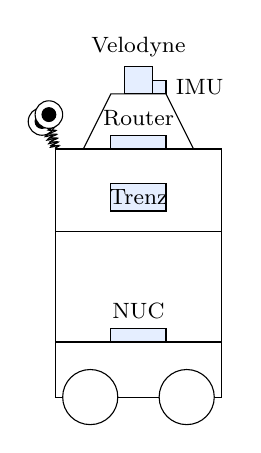
\begin{tikzpicture}[scale=0.35]
\draw (0, 0) rectangle (6, 3);
\draw (1, 3) -- (2, 5) -- (4, 5) -- (5, 3);
\draw [fill=light] (2, 0.75) rectangle +(2, 1);
\node at (3, 1.25) {\footnotesize Trenz};
\draw [fill=light] (2, 3) rectangle +(2, 0.5);
\node [above] at (3, 3.5) {\footnotesize Router};
\draw [fill=light] (2.5, 5) rectangle +(1, 1);
\node [above] at (3, 6) {\footnotesize Velodyne};
\draw (0, 0) -- (0, -6) -- (6, -6) -- (6, 0);
\draw [fill=light] (3.5, 5) rectangle +(0.5, 0.5);
\node [right] at (4, 5.25) {\footnotesize IMU};
\draw (0, -4) -- (6, -4);
\draw [fill=light] (2, -4) rectangle +(2, 0.5);
\node [above] at (3, -3.5) {\footnotesize NUC};
%\draw [fill=light] (2.5, -6) rectangle +(1, 0.5);
%\node [above] at (3, -5.5) {\footnotesize IMU};
\draw [fill=white] (1.25, -6) circle (1);
\draw [fill=white] (4.75, -6) circle (1);
\draw [decorate, decoration={snake, segment length=0.5mm, amplitude=0.5mm}] (-0.5, 4) -- (0, 3);
\draw [fill=white] (-0.5, 4) circle (0.5);
\draw [fill=black] (-0.5, 4) circle (0.25);
\draw [decorate, decoration={snake, segment length=0.5mm, amplitude=0.5mm}] (-0.25, 4.25) -- (0, 3);
\draw [fill=white] (-0.25, 4.25) circle (0.5);
\draw [fill=black] (-0.25, 4.25) circle (0.25);
\end{tikzpicture} &
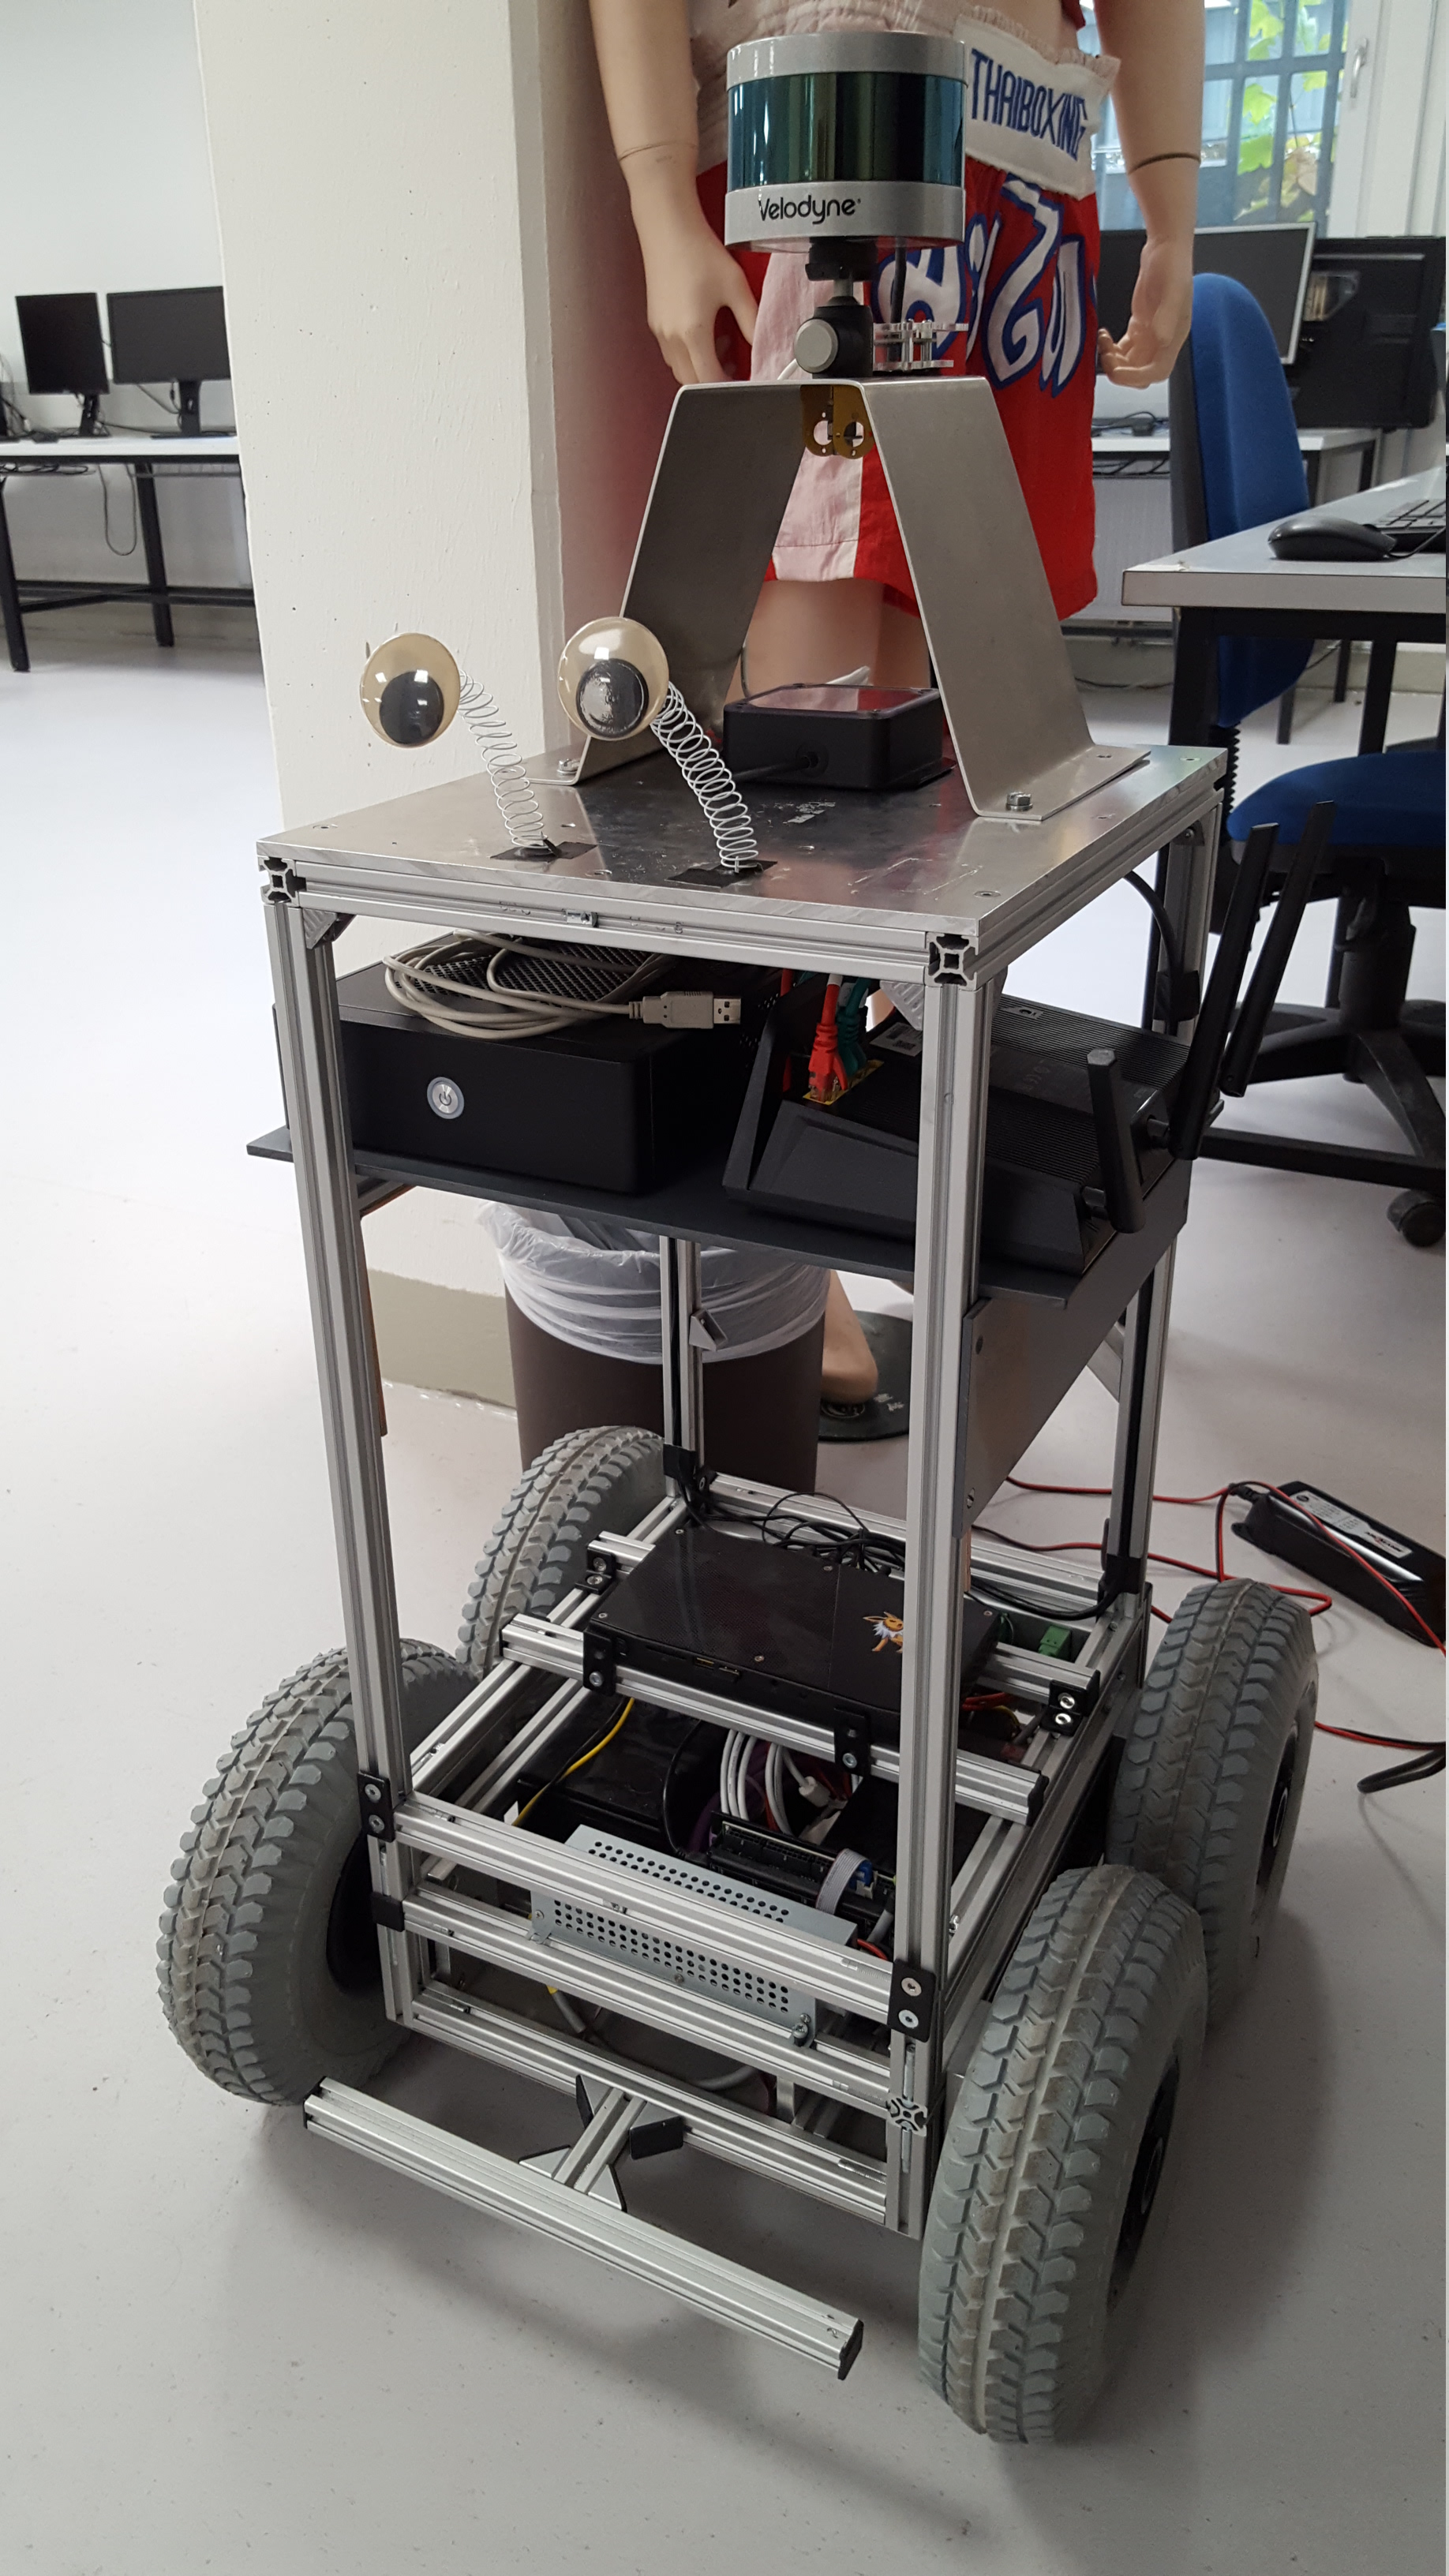
\includegraphics[height=5cm]{images/robot.jpg}
\end{tabular}
\end{center}

\begin{itemize}
\item{Grundlegender Hardware Accelerated TSDF SLAM Algorithmus fertig}
\item{Zeit: 0,87\,fps} % = 1 / (35ms + 676ms + 105ms + 337ms)
\item{Power Consumption: 10,32\,W}
\item{Verbesserungspotenzial vorhanden}
\end{itemize}
\end{frame}

\section{Ziele für MS\,3}
\begin{frame}{\secname}
\begin{textblock*}{12cm}(1cm,2cm)
\begin{itemize}
\item{Aufbau einer SLAM-Box}
\begin{itemize}
\item{Nutzung als Sensor}
\item{Einfache Portierung zwischen Drohne, Roboter, Rucksack etc.}
\item{Festes Interface, einfache Bedienung, Kapselung}
\end{itemize}
\end{itemize}
\end{textblock*}
\begin{textblock*}{12cm}(1cm,3.9cm)
\begin{itemize}
\item{Verbesserung und Optimierung des Algorithmus \\
\vspace{0.2cm}
\begin{tabular}{ll}
\toprule
Variable & Ziel \\
\midrule
Genauigkeit & Wiederfinden erneuter Pose \\
Energie & 0,5\,J/frame \\
Frequenz & \textbf{20\,fps} (echtzeitfähig) \\
Geschwindigkeit & 10\,km/h \\
\bottomrule
\end{tabular}}
\end{itemize}
\end{textblock*}
\begin{textblock*}{12cm}(1cm,7.7cm)
\begin{itemize}
\item{Mesh-Generierung auf Basis der TSDF Werte}
\end{itemize}
\end{textblock*}
\end{frame}

\section{Was haben wir wirklich gemacht?}
\begin{frame}{\secname}
\begin{textblock*}{12cm}(1cm,2cm)
\begin{itemize}
\item{Aufbau einer SLAM-Box {\small\color{dark}$\rightarrow$ \textbf{Aufbau}}}
\begin{itemize}
\item{Nutzung als Sensor}
\item{\sout{Einfache Portierung zwischen Drohne, Roboter, Rucksack etc.}}
\item{Festes Interface, einfache Bedienung, Kapselung}
\end{itemize}
\end{itemize}
\end{textblock*}
\begin{textblock*}{12cm}(1cm,3.9cm)
\begin{itemize}
\item{Verbesserung und Optimierung des Algorithmus}
\begin{itemize}
\item[$\rightarrow$]{\color{dark} \textbf{Base Design}}
\item[$\rightarrow$]{\color{dark} \textbf{Kommunikation}}
\item[$\rightarrow$]{\color{dark} \textbf{Preprocessing}}
\item[$\rightarrow$]{\color{dark} \textbf{Registrierung vollständig auf Hardware}}
\item[$\rightarrow$]{\color{dark} \textbf{Asynchrones TSDF Update}}
\end{itemize}
\end{itemize}
\end{textblock*}
\begin{textblock*}{12cm}(1cm,7.7cm)
\begin{itemize}
\item{Mesh-Generierung auf Basis der TSDF Werte}
\begin{itemize}
\item[$\rightarrow$]{\color{dark} \textbf{Mesh Rekonstruktion}}
\end{itemize}
\end{itemize}
\end{textblock*}
\end{frame}

\subsection{Drohne, Laserscanner}
\begin{frame}{\subsecname}
\begin{itemize}
\item{Drohne erfordert neuen Laserscanner}
\begin{itemize}
\item{Velodyne nicht geeignet}
\end{itemize}
\item{Kontakt mit Firmen:}
\begin{itemize}
\item{Ouster}
\item{Blickfeld}
\end{itemize}
\item[$\rightarrow$]{Nicht erfolgreich}
\end{itemize}
\begin{textblock*}{4cm}(8cm,2cm)
\centering
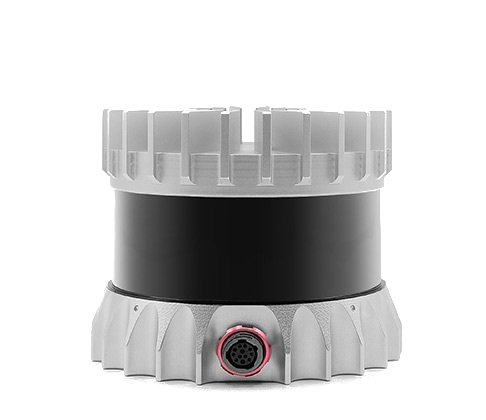
\includegraphics[width=4cm]{images/ouster.png}
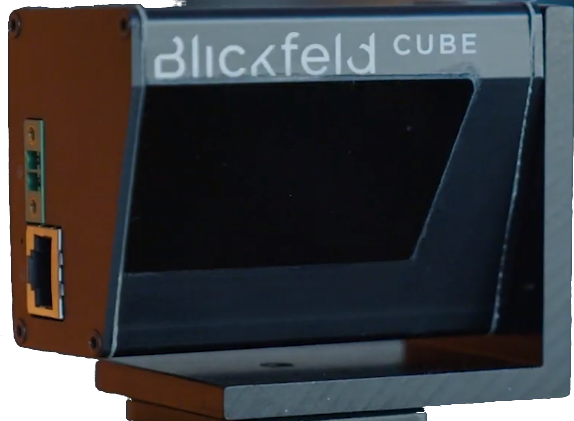
\includegraphics[width=3cm]{images/blickfeld.png}
\end{textblock*}
\end{frame}

\subsection{Aufbau}
\begin{frame}{\subsecname}
TODO
\end{frame}

\subsection{Base Design}
\begin{frame}{\subsecname}
TODO

Experte Marcel
\end{frame}

\subsection{Kommunikation}
\begin{frame}{\subsecname}
TODO

Experte Julian
\end{frame}

\subsection{Algorithmus}

\subsubsection*{Preprocessing}
\begin{frame}{\subsecname: \subsubsecname}
\begin{tabular}{m{4cm}m{6cm}}
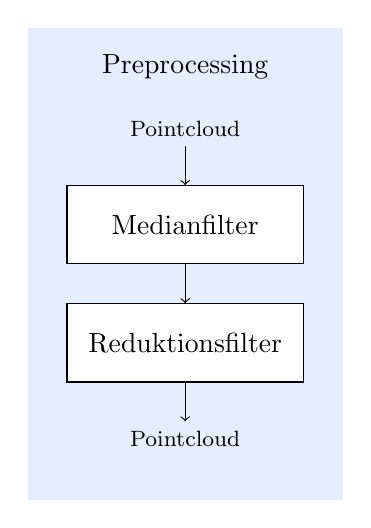
\begin{tikzpicture}
\fill[light] (0, 0) rectangle (4, 6);
\node at (2, 5.5) {Preprocessing};
\draw[->] (2, 4.5) node[above] {\footnotesize Pointcloud} -- (2, 4);
\draw[fill=white] (0.5, 3) rectangle +(3, 1) node[pos=0.5] {Medianfilter};
\draw[->] (2, 3) -- (2, 2.5);
\draw[fill=white] (0.5, 1.5) rectangle +(3, 1) node[pos=0.5] {Reduktionsfilter};
\draw[->] (2, 1.5) -- (2, 1) node[below] {\footnotesize Pointcloud};
\end{tikzpicture} &
\begin{itemize}
\item{TODO (Pascal) Verschiedene Filter?}
\end{itemize}
\end{tabular}
\end{frame}

\subsubsection*{Registrierung}
\begin{frame}{\subsecname: \subsubsecname}
TODO

Experten Malte, Patrick
\end{frame}

\subsubsection*{Asynchronität}
\begin{frame}{\subsecname: \subsubsecname}
\begin{textblock*}{12.8cm}(0cm, 1.1cm)
\centering
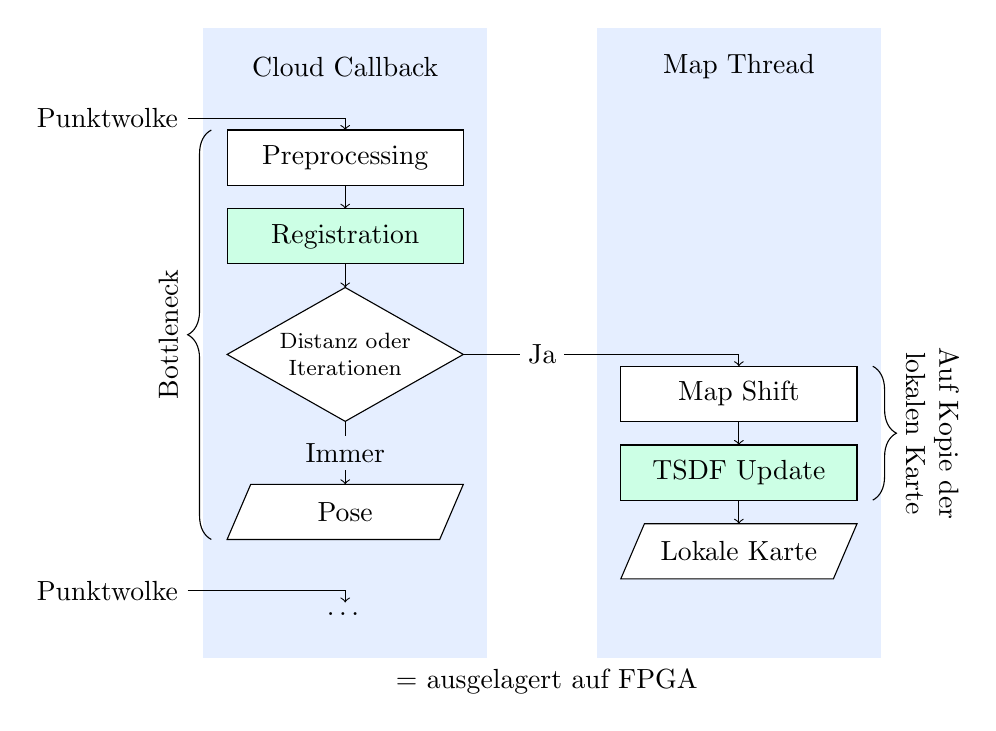
\begin{tikzpicture}
\fill[light] (-0.3, 1) rectangle (3.3, 9);
\fill[light] (4.7, 1) rectangle (8.3, 9);
\node at (1.5, 8.5) {Cloud Callback};
\node at (6.5, 8.5) {Map Thread};
\draw[->] (-0.5, 7.85) node[left] {Punktwolke} -- (1.5, 7.85) -- (1.5, 7.7);
\draw[fill=white] (0, 7) rectangle +(3, 0.7) node[pos=0.5] {Preprocessing};
\draw[->] (1.5, 6) -- (1.5, 5.7);
\draw[fill=hw] (0, 6) rectangle +(3, 0.7) node[pos=0.5] {Registration};
\draw[->] (1.5, 7) -- (1.5, 6.7);
\draw[fill=white] (0, 4.85) -- (1.5, 4) -- (3, 4.85) -- (1.5, 5.7) -- cycle;
\node at (1.5, 4.85) {\begin{minipage}{2cm}\centering\footnotesize Distanz oder\\Iterationen\\\end{minipage}};
\draw[->] (1.5, 4) -- (1.5, 3.2) node[midway, fill=light, inner sep=0.1cm] {Immer};
\draw[fill=white] (0, 2.5) -- (2.7, 2.5) -- (3, 3.2) -- (0.3, 3.2) -- cycle;
\node at (1.5, 2.85) {Pose};
\draw[->] (3, 4.85) -- (6.5, 4.85) -- (6.5, 4.7);
\node[fill=white, inner sep=0.1cm] at (4, 4.85) {Ja};
\draw[fill=white] (5, 4) rectangle +(3, 0.7) node[pos=0.5] {Map Shift};
\draw[->] (6.5, 3) -- (6.5, 2.7);
\draw[fill=hw] (5, 3) rectangle +(3, 0.7) node[pos=0.5] {TSDF Update};
\draw[->] (6.5, 4) -- (6.5, 3.7);
\draw[fill=white] (5, 2) -- (7.7, 2) -- (8, 2.7) -- (5.3, 2.7) -- cycle;
\node at (6.5, 2.35) {Lokale Karte};
\draw[->] (-0.5, 1.85) node[left] {Punktwolke} -- (1.5, 1.85) -- (1.5, 1.7) node[below] {\dots};
\draw [decorate, decoration={brace, amplitude=0.3cm, mirror}]
(-0.2, 7.7) -- (-0.2, 2.5) node[midway, xshift=-0.3cm, above, rotate=90] {Bottleneck};
\draw [decorate, decoration={brace, amplitude=0.3cm}]
(8.2, 4.7) -- (8.2, 3) node[midway, xshift=0.3cm, above, rotate=270]
{\begin{minipage}{4cm}\centering Auf Kopie der\\lokalen Karte\\\end{minipage}};
\node at (4, 0.7) {{\color{hw}$\blacksquare$} = ausgelagert auf FPGA};
\end{tikzpicture}
\end{textblock*}
\end{frame}

\subsection{Mesh Rekonstruktion}
\begin{frame}{\subsecname}
\begin{itemize}
\item{Global Map offline}
\begin{itemize}
\item{Programm im LVR2 Repository}
\item{Mesh Verbesserungen}
\item{HDF5 $\rightarrow$ PLY}
\end{itemize}
\item{Local Map online}
\begin{itemize}
\item{ROS Node}
\item{Marker Message $\rightarrow$ Mesh Message}
\end{itemize}
\end{itemize}

\begin{center}
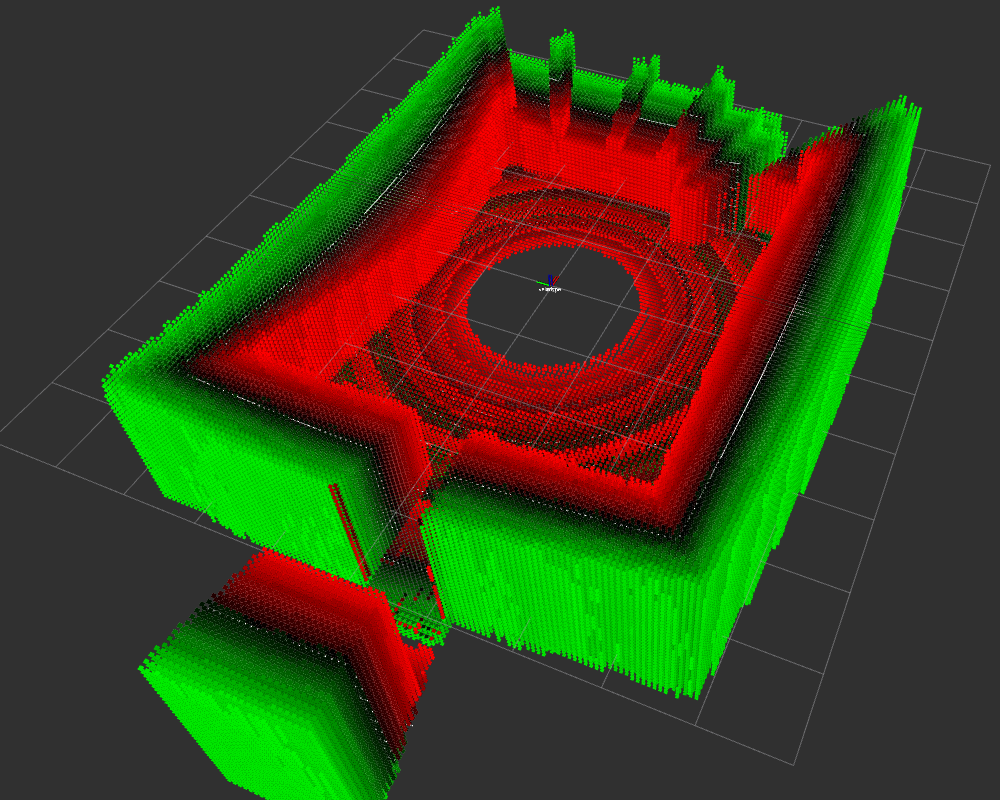
\includegraphics[width=5cm]{images/ReconstructionTSDF.png}
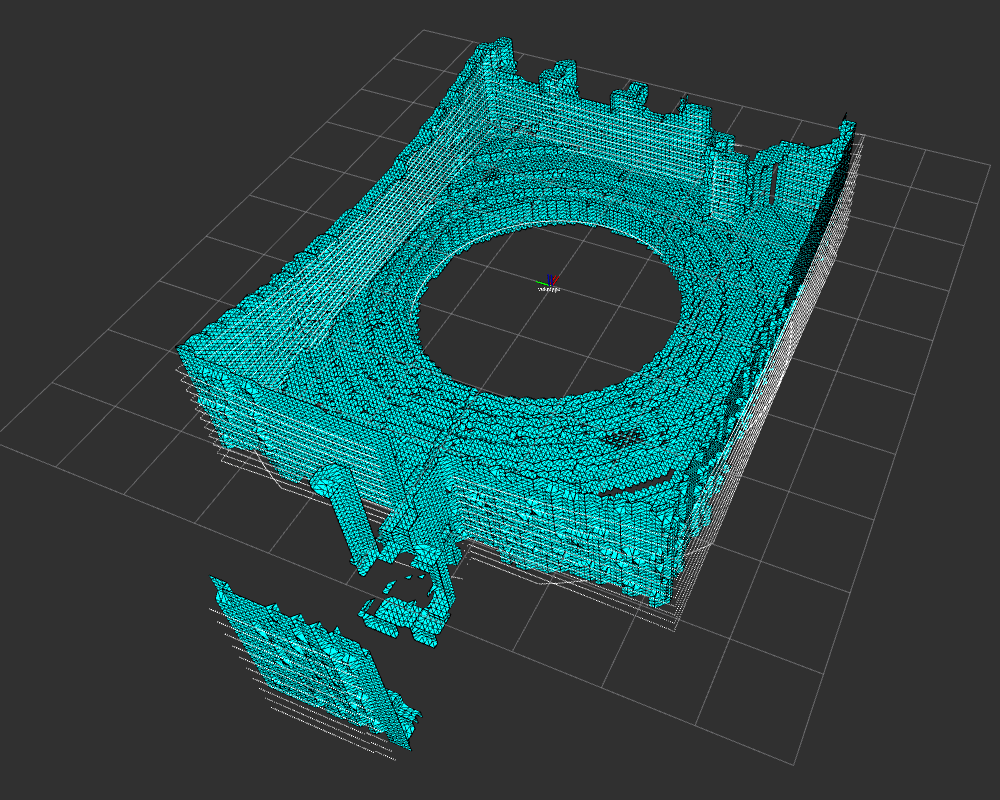
\includegraphics[width=5cm]{images/ReconstructionMesh.png}
\end{center}
\end{frame}

\subsection{Paper}
\begin{frame}{\subsecname}
\centering
\begin{tikzpicture}[scale=0.8]
\draw[thick] (-4, 0) rectangle +(2, 5.4);
\node at (-3, 0.5) {\begin{minipage}{2cm}\centering\footnotesize
External\\
ROS Nodes\\
\end{minipage}};

\draw[fill=light] (-3.8, 3.2) rectangle +(1.6, 2) node[pos=0.5] {\begin{minipage}{1.6cm}\centering
%Sensors\\
%\begin{footnotesize}
%Lidar\\
%IMU\\
%Camera\\
%\dots\\
%\end{footnotesize}
\end{minipage}};

\draw[fill=light] (-3.8, 1) rectangle +(1.6, 2) node[pos=0.5] {\begin{minipage}{1.6cm}\centering
%Control\\
%\begin{footnotesize}
%Motor\\
%Battery\\
%\dots\\
%\end{footnotesize}
\end{minipage}};

\draw (0.2, 1.4) rectangle +(6.4, 3.8);
\node at (3.4, 4.9) {\footnotesize Reconfigurable System on Chip};
\node at (3.56, 0.66) {\includegraphics[height=0.96cm]{images/pynq.png}};
\draw (0.2, 1.4) -- (3.1, 0.7);
\draw (6.6, 1.4) -- (3.7, 0.7);
\draw[dark, ultra thick] (3.4, 0.7) circle (0.3);

\draw[fill=light] (0.4, 1.6) rectangle +(2, 3);
\node at (1.4, 4.1) {\footnotesize Processor};
\draw (0.5, 3.1) rectangle +(1.8, 0.5);% node[pos=0.5] {\footnotesize ROS Master};
\draw (0.5, 2.5) rectangle +(1.8, 0.5);% node[pos=0.5] {\tiny Motor Ctrl Node};
\draw (0.5, 1.9) rectangle +(1.8, 0.5);% node[pos=0.5] {\tiny SLAM Node};
%\node at (1.4, 1.75) {\footnotesize \dots};

\draw[shade, left color=light, right color=hw] (2.6, 1.6) rectangle +(1.6, 3);
\node at (3.4, 4.1) {\begin{minipage}{1.6cm}\centering\footnotesize
Shared\\
Memory\\
\end{minipage}};

\draw[fill=hw] (4.4, 1.6) rectangle +(2, 3);
\node at (5.4, 4.1) {\footnotesize FPGA};

\node at (-1, 3.1) {\begin{minipage}{2cm}\centering\footnotesize
ROS\\
Messages\\
\end{minipage}};
\draw[<->] (-2.2, 3.8) -- (0.4, 3.8);
\draw[<->] (-2.2, 2.4) -- (0.4, 2.4);

\draw[thick] (0, 0) rectangle +(6.8, 5.4);
\node[left] at (6.8, 0.3) {\footnotesize ReconfROS};

% Shared Memory
\draw (2.9, 3.15) rectangle +(1, 0.4);
\draw (2.9, 2.55) rectangle +(1, 0.4);
\draw (2.9, 1.95) rectangle +(1, 0.4);

% FPGA
\draw (4.5, 3.1) rectangle +(1.8, 0.5);% node[pos=0.5] {\tiny Path Detection};
\draw (4.5, 2.5) rectangle +(1.8, 0.5);% node[pos=0.5] {\tiny Registration};
\draw (4.5, 1.9) rectangle +(1.8, 0.5);% node[pos=0.5] {\tiny Outlier Removal};
%\node at (5.4, 1.75) {\footnotesize \dots};

\draw[<->] (2.3, 2.75) -- (2.9, 3.35);
\draw[<->] (2.3, 2.15) -- (2.9, 2.75);
\draw[<->] (2.3, 2.15) -- (2.9, 2.15);
\draw[<->] (3.9, 3.35) -- (4.5, 3.35);
\draw[<->] (3.9, 2.75) -- (4.5, 2.75);
\draw[<->] (3.9, 2.15) -- (4.5, 2.15);
\end{tikzpicture}

\vspace{0.3cm}

\begin{tikzpicture}[scale=0.7]
\setlength{\fboxsep}{0pt}
\node[inner sep=0pt] at (0, 5) {\fbox{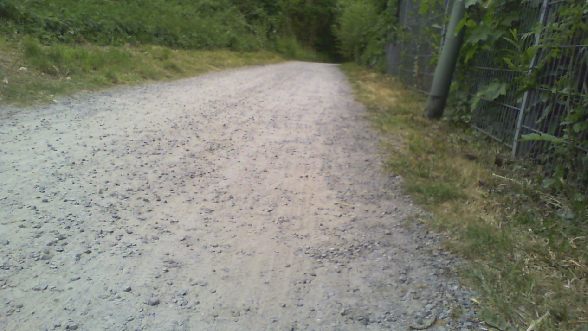
\includegraphics[width=2.1cm]{images/pipeline_pics/cam.png}}};
\node at (0, 3.75) {\footnotesize Camera image};
\node[inner sep=0pt] at (4, 5) {\fbox{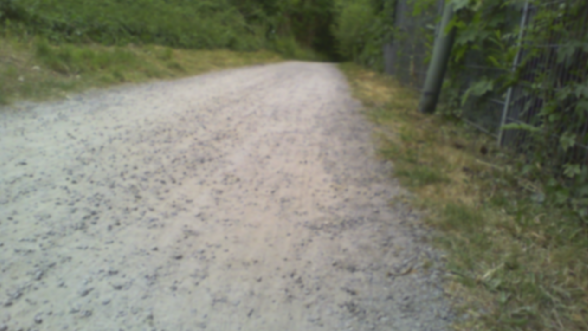
\includegraphics[width=2.1cm]{images/pipeline_pics/gauss.png}}};
\node at (4, 3.75) {\footnotesize Removing noise};
\node[inner sep=0pt] at (8, 5) {\fbox{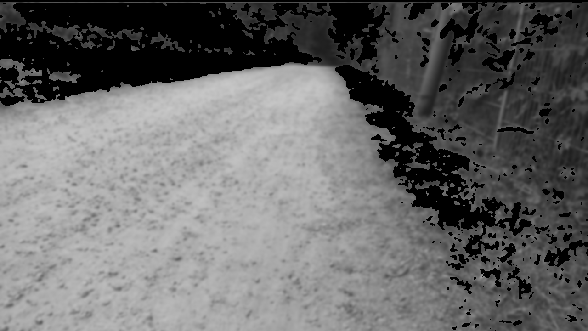
\includegraphics[width=2.1cm]{images/pipeline_pics/green_filter.png}}};
\node at (8, 3.75) {\footnotesize Trail pixel extraction};
\node[inner sep=0pt] at (0, 2) {\fbox{
\includegraphics[width=2.1cm]{images/pipeline_pics/threshold.png}}};
\node at (0, 0.75) {\footnotesize Thresholding};
\node[inner sep=0pt] at (4, 2) {\fbox{
\includegraphics[width=2.1cm]{images/pipeline_pics/morph.png}}};
\node at (4, 0.75) {\footnotesize Remove fragments};
\node[inner sep=0pt] at (8, 2) {\fbox{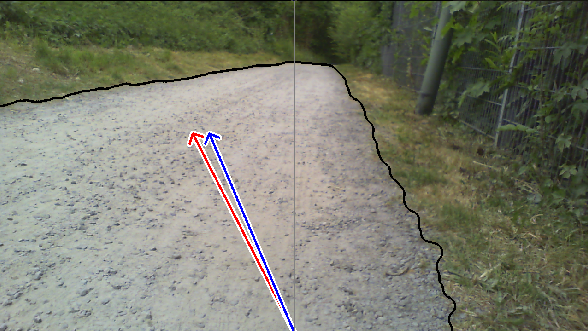
\includegraphics[width=2.1cm]{images/pipeline_pics/direction.png}}};
\node at (8, 0.75) {\footnotesize Trail direction};
\draw[->] (1.5, 5) -- (2.5, 5);
\draw[->] (5.5, 5) -- (6.5, 5);
\draw[->] (9.5, 5) -- (10, 5) -- (10, 3.25) -- (-2, 3.25) -- (-2, 2) -- (-1.5, 2);
\draw[->] (1.5, 2) -- (2.5, 2);
\draw[->] (5.5, 2) -- (6.5, 2);
\end{tikzpicture}
\end{frame}

\section{Evaluation}

\subsection{Zeit}
\begin{frame}{\secname: \subsecname}
TODO
\end{frame}

\subsection{Power Consumption}
\begin{frame}{\secname: \subsecname}
TODO
\end{frame}

\subsection{Qualität}
\begin{frame}{\secname: \subsecname}
TODO
\end{frame}

\section{Ausblick}
\begin{frame}{\secname}
\begin{itemize}
\item{FastSense Paper}
\item{Loop Closing}
\item{Drohne}
\item{Modulares Design}
\item{Grillen bei Mario}
\end{itemize}
\end{frame}

\begin{frame}{Ende}
\centering\LARGE
Vielen Dank für Eure Aufmerksamkeit!\\\vspace{1cm}
Fragen?
\end{frame}

\end{document}
